\chapter{Developping a DBMS Transactional Testing Framework}

\section{Overview}

This chapter presents the design, implementation and usage of a testing framework for replicating DBMS transactional bugs. Using the testing framework, we replicate a set of transactional bugs in the \textit{MySQL}, \textit{MariaDB} and \textit{TiDB} DBMSs. We then analyse the reports of the replicated bugs, and we explore the corelation between isolation levels and the reported bugs.

\section{Design}

The testing framework, is implemented in \textit{Python}, and heavily relies on \textit{Podman}, a container manager \cite{podmanwebpage} for managing DBMS instances. The tool works on \code{x64 GNU/Linux} systems, and we developped it in \textit{VSCode}, with the help of \textit{Github Copilot} \cite{copilotwebpage}.


\begin{figure}[!h]
    \centering
    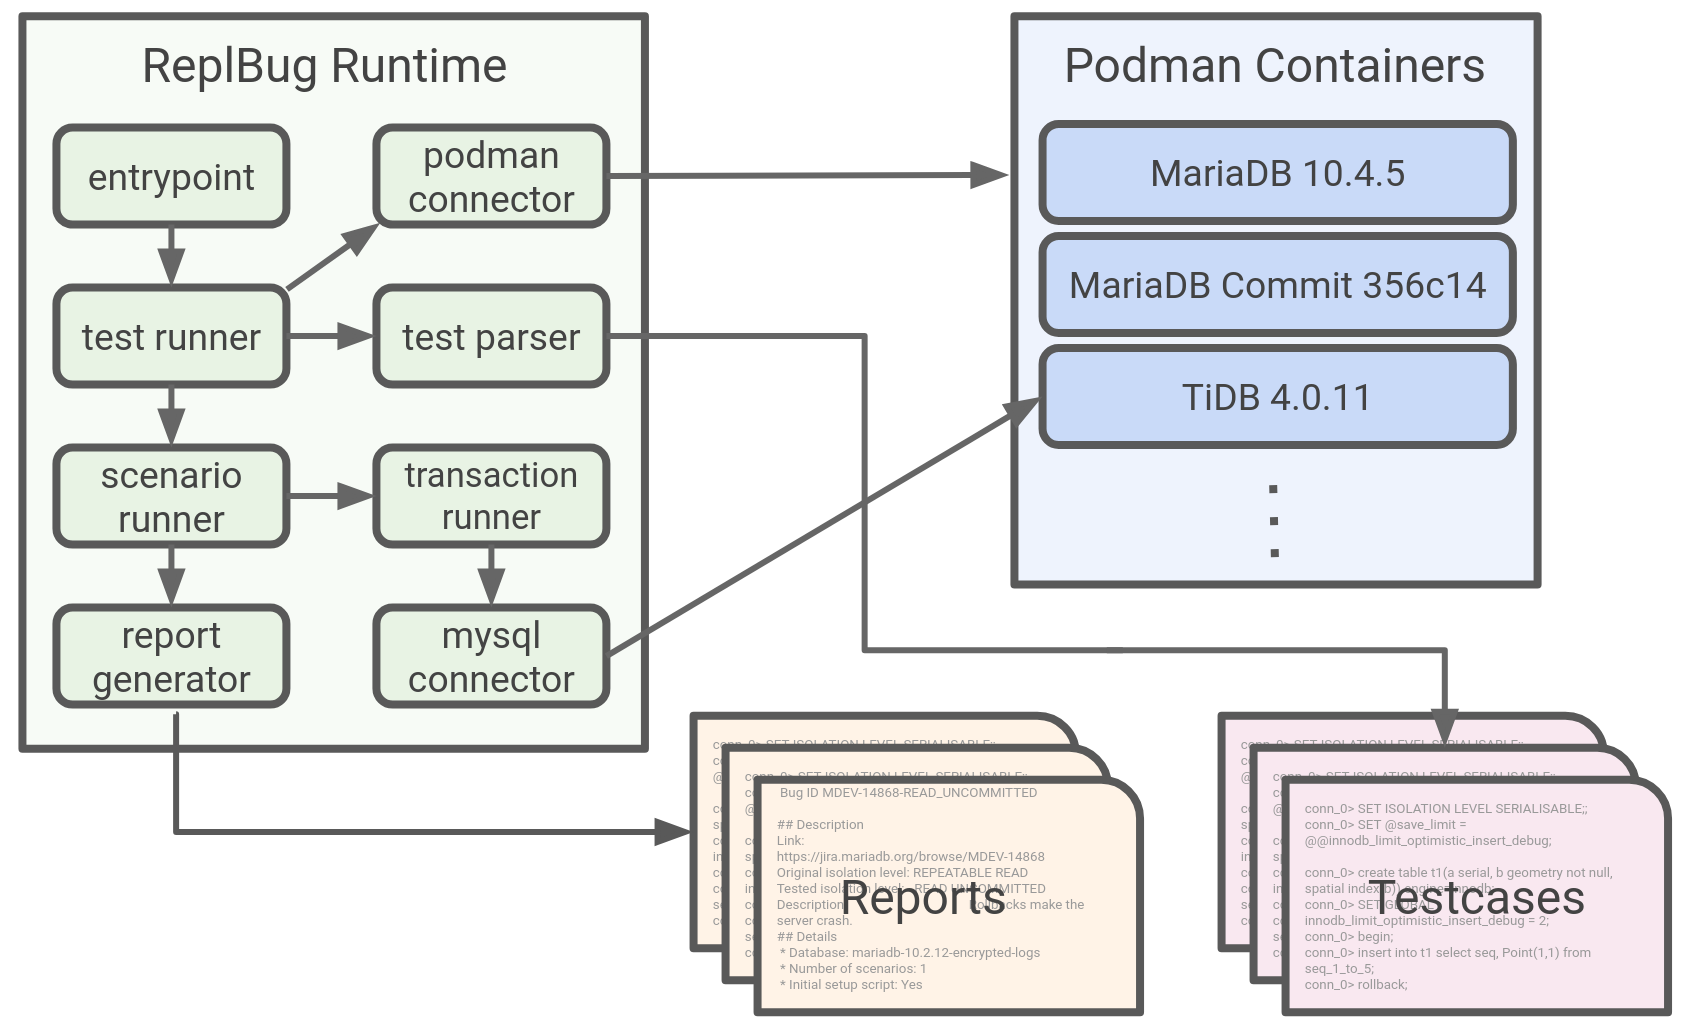
\includegraphics[width=\linewidth]{assets/replbug_design.png}
    \caption{Design of the \textit{ReplBug} testing framework}
    \label{fig:replb_design}
\end{figure}


The framework is modular, helping any future developer to easily extend it (for instance for adding support for new DBMSs). The main components in the bug testing pipeline (see Figure \ref{fig:replb_design}) are the following:

\begin{itemize}
    \item The \textit{podman connector}: This component handles the interaction with the \textit{Podman} engine, and is responsible for starting, stopping, downloading and managing containers running DBMS instances.
    \item The \textit{test parser}: This component handles the parsing of testcases, using a specific format, and is responsible for creating the internal representation of the testcases.
    \item The \textit{mysql connector}: This component handles the connection to a DBMS instance (running within a container), and is responsible for executing statements in order and extracting the results.
    \item The \textit{transaction runner}: This component handles the execution of all the statements in a transaction, and runs on different threads for concurrency.
    \item The \textit{scenario runner}: This component runs testcases under a specific configuration.
    \item The \textit{test runner}: This component orchestrates the execution of all required testcases under all specified configurations. 
\end{itemize}

\section{Custom DBMS Version}

Some bugs are specific to a certain version of a DBMS, which might not be available as pre-built binaries. For instance, versions with serious vulnerabilities are usually removed from official repositories, or intermediary versions tied to a specifig \textit{Git} commit are not released as binaries.

For the mentioned reasons, we consider the ability to built DBMSs from source essential. To simplify the process, we provide sample \textit{Dockerfile} templates, which can be used to test specific DMBS versions. A sample \textit{Dockerfile} for \textit{TiKV} can be seen in Figure \ref{fig:dockerfilesample}.
 
\begin{figure}
\begin{minted}[bgcolor=bg]{Dockerfile}
FROM golang:1.19-alpine AS builder

# Install git and other dependencies
RUN apk add --no-cache git make bash gcc wget binutils-gold \
    musl-dev curl tar

# Set the working directory inside the container and
# create necessary directories
RUN mkdir -p /go/src/github.com/pingcap
WORKDIR /go/src/github.com/pingcap

ARG TIDB_COMMIT=c9288d246c99073ff04304363dc7234d9caa5090

# Clone and build the TiDB repository
RUN git clone --depth 1 https://github.com/pingcap/tidb.git \
    && cd tidb \
    && git fetch --depth 1 origin "$TIDB_COMMIT" \
    && git checkout "$TIDB_COMMIT" \
    && make -j \
    && mv bin/tidb-server /usr/local/bin/tidb-server \
    && cd .. \
    && rm -rf tidb

EXPOSE 4000
WORKDIR /usr/local/bin
CMD ["./tidb-server", "-P", "4000"]    
\end{minted}
\caption{Sample \textit{Dockerfile} for building a specific version of \textit{TiDB}}
\label{fig:dockerfilesample}
\end{figure}

In our project, we provide \textit{Dockerfiles} for \textit{MySQL}, \textit{MariaDB} in release or debug mode, and \textit{TiDB} with or without \textit{TiKV}. Creating a new docker file only requires the \textit{Git} commit, and then running the \textit{build} command integrated into \textit{ReplBug}. 

\section{Testing Meta-Language}

For a given testcase, specifying the statements and their execution order on the DBMS is hard, due to multiple reasons:
\begin{itemize}
    \item Transactional and isolation bug PoCs usually need multiple concurent transactions, making a simple \textit{SQL} script insufficient.
    \item Some statements are expected to fail, which might lead to the termination of a standard script.
    \item The order of the statement execution (and sometimes the locking order) is important for the bug to manifest.
\end{itemize} 

To address these issues, the \textit{MySQL} development team created a testing framework which encodes testcases in a special format \cite{mysqltestrun}. Using this format, however, is cubersome, as we only need a small subset of the features, and using the \textit{MySQL} interpreter would make it hard to test other DBMSs. 

We thus create a small, custom scripting language on top of \textit{Python}, inspired by the way bug reporters describe their PoCs. In Figure \ref{fig:bug_metalanguage_sample}, we present a sample testcase for the bug \textit{MDEV-26642} in \textit{MariaDB 10.6.17}.

\begin{figure}
\begin{minted}[bgcolor=bg]{Python}
ORIGINAL_ISOLATION_LEVEL = DEFAULT_ISOLATION_LEVEL
BUG_ID = "MDEV-26642"
LINK = "https://jira.mariadb.org/browse/MDEV-26642"
DB_AND_VERSION = db_config.DatabaseTypeAndVersion(
    db_config.DatabaseType.MARIADB, "10.6.17"
)
SETUP_SQL_SCRIPT = """
create table t(a int, b int);
insert into t values (0, 0), (1, 1), (2, 2);
"""

DESCRIPTION = "The last select does not respect the update
                (a should always be 10)."


def get_scenarios(isolation_level: IsolationLevel):
    return [
        f"""
        conn_0> SET GLOBAL TRANSACTION ISOLATION LEVEL
                                {isolation_level.value};
        conn_0> begin;
        conn_0> select * from t;
        conn_1> begin;
        conn_1> update t set a = 10 where b = 1;
        conn_1> commit;
        conn_0> select * from t;
        conn_0> update t set a = 10 where true;
        conn_0> select * from t;
        conn_0> commit;
        """,
    ]
\end{minted}
\caption{Replication script for the bug \textit{MDEV-26642} in \textit{MariaDB 10.6.17}.} \label{fig:bug_metalanguage_sample}
\end{figure}

Each testcase provides the following information:
\begin{itemize}
    \item The \textit{DBMS} and version on which the bug was reported.
    \item The bug ID and a link to the bug report.
    \item The setup script, which is executed before the testcases. If the setup script is too long, it can be stored in a separate file.
    \item The description of the bug.
    \item The scenarios, which are the testcases that will be executed (one for each isolation level). Each scenario is a sequence of statements, executed in parallel by different connections.
\end{itemize}

For running a testcase, the tool provisions the required DBMS instance, executes the setup script (if present), and then runs the scenarios under all supported isolation levels. For each transaction a separate connection to the DBMS server is created. The results are then stored in a report, which can be further analysed.

\section{Usage}



\begin{figure}
    \centering
    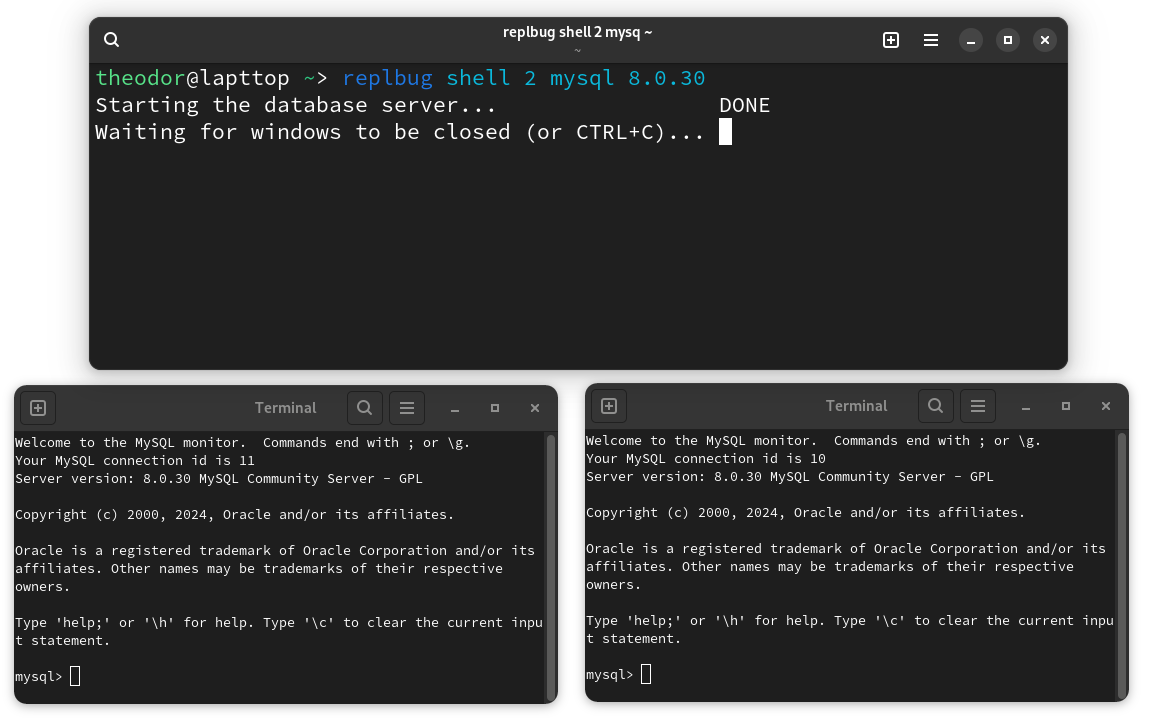
\includegraphics[width=\linewidth]{assets/replbug_shell.png}
    \caption{Using \textit{ReplBug} to start 2 \textit{MySQL v8.0.30} shells}
    \label{fig:replb_shell}
\end{figure}

\begin{figure}
    \centering
    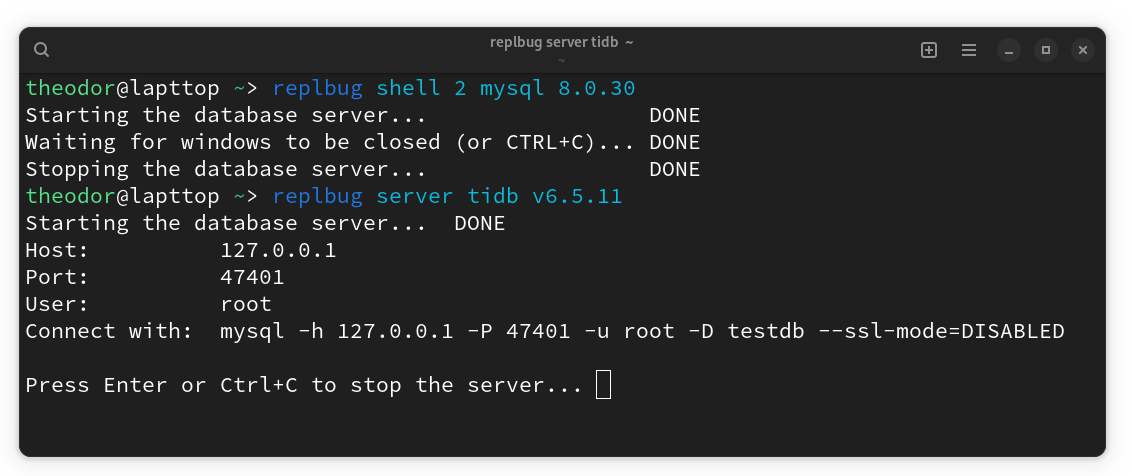
\includegraphics[width=\linewidth]{assets/replbug_server.png}
    \caption{Using \textit{ReplBug} to start a \textit{TiDB v6.5.11} server}
    \label{fig:repl_server}
\end{figure}

\begin{figure}
    \centering
    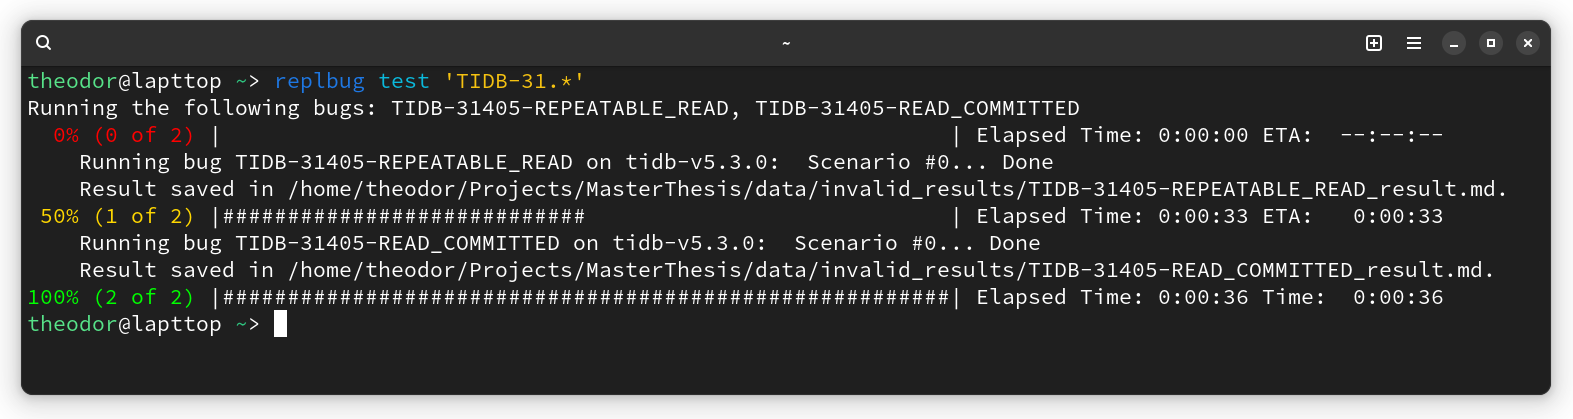
\includegraphics[width=\linewidth]{assets/replbug_test.png}
    \caption{Using \textit{ReplBug} to generate reports of some known bugs}
    \label{fig:repl_test}
\end{figure}


\begin{figure}
    \centering
    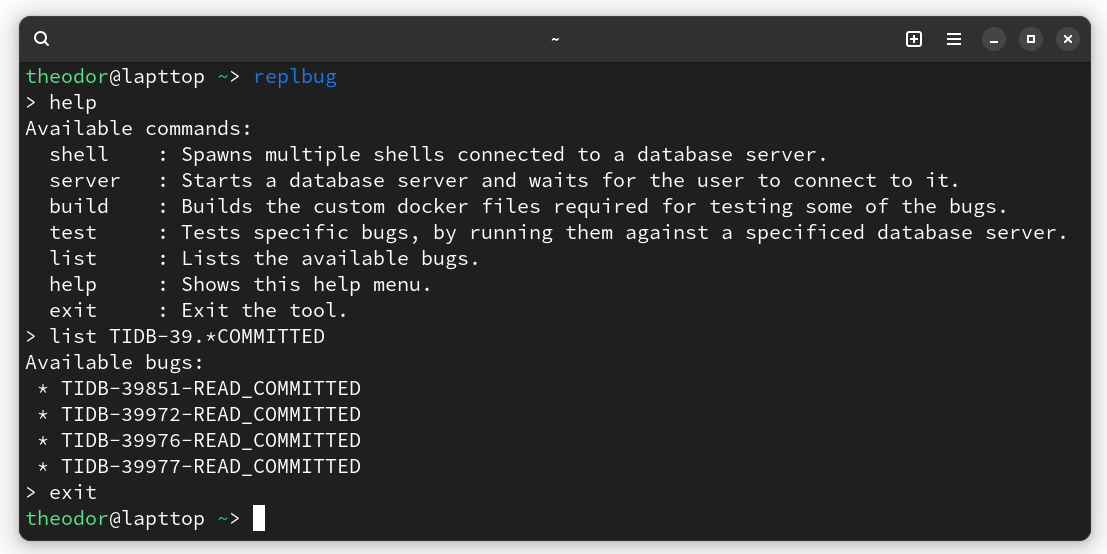
\includegraphics[width=\linewidth]{assets/replbug_interactive.png}
    \caption{Using \textit{ReplBug} in interactive mode}
    \label{fig:repl_interactive}
\end{figure}




The testing framework, called \textit{ReplBug} is invoked from the CLI. The main features it offers, exposed by the executable as subcommands are the following:
\begin{itemize}
    \item \textbf{\code{shell}} (See Figure \ref{fig:replb_shell}): Starts one or multiple \textit{MySQL}, \textit{MariaDB} or \textit{TiDB} shells, connected to a specific version of the DBMS. If the version is not present on the local machine, the tool will attempt to pull the image from Docker Hub.
    \item \textbf{\code{server}} (See Figure \ref{fig:repl_server}): Starts a specific version of the \textit{MySQL}, \textit{MariaDB} or \textit{TiDB} DBMS and provides the required details (host, port, user) for connecting to the server.
    \item \textbf{\code{test}} (See Figure \ref{fig:repl_test}): Runs the scenarios of some known bugs (which have to be written in a specific format prior), and automatically generates reports of the execution.
    \item \textbf{\code{list}}: Returns a list of the testcases available in the tool (optionally a \textit{regex} can be passed to filter the results).
\end{itemize}

The tool can be either used from the CLI by passing arguments, or in interactive mode, where the tool exposes a shell that can be used by the user  (see Figure \ref{fig:repl_interactive}).

\chapter{Replicating Transactional Bugs in MySQL, MariaDB and TiDB}

\section{Overview}

With the help of the \textit{ReplBug} testing framework, we were able to replicate \textit{MySQL}, \textit{MariaDB} and \textit{TiDB} transactional, logical and isolation bugs. We focus on transaction and isolation bugs, reported by DBMS testing papers \cite{cui2024understanding_ICSE2024, dou2023detecting_ICSE2023, cui2022differentially_ASE2022}. We then replicate the bugs on the same versions of the DBMSs, and verify which isolation levels are affected. The number of bugs taken from each paper can be seen in Figure \ref{fig:bugs_by_paper}.


\begin{figure}
    \centering
    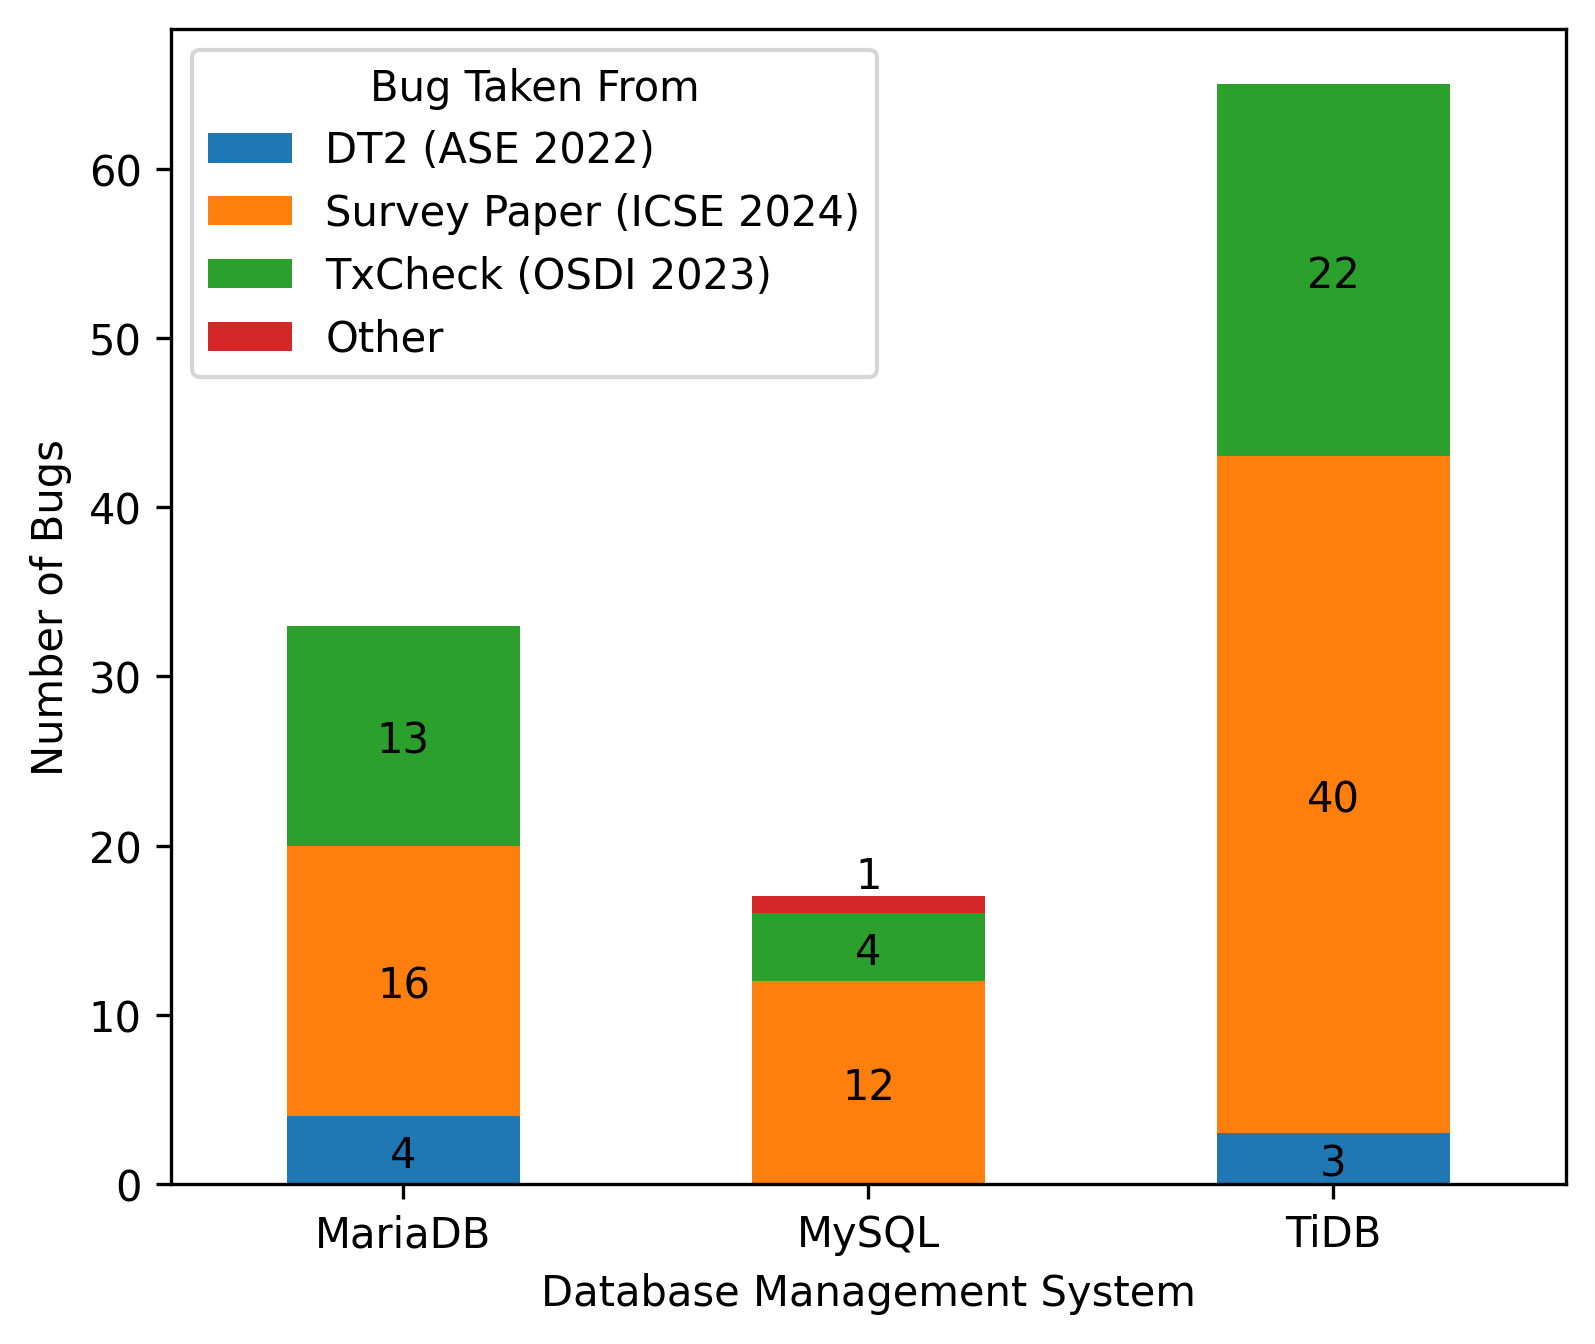
\includegraphics[width=0.7\linewidth]{assets/bug_replication_bugs_by_dbms_and_paper.png}
    \caption{Distribution of bugs by DBMS and reporting paper  \cite{cui2024understanding_ICSE2024, dou2023detecting_ICSE2023, cui2022differentially_ASE2022}.}
    \label{fig:bugs_by_paper}
\end{figure}

We try to replicate \textit{MySQL} and \textit{MariaDB} bugs on the $4$ isolation levels supported by the DBMSs (\textit{Read Uncommitted}, \textit{Read Committed}, \textit{Repeatable Read} and \textit{Serializable}). For \textit{TiDB}, we replicate the bugs on the $2$ isolation levels supported by the DBMS (\textit{Read Committed} and \textit{Serializable}).

